\bigskip

\item Which of the following is the approximate value for the sine and cosine of angles $A$ and $B$ in the figure below.

% \resizebox{3in}{!}{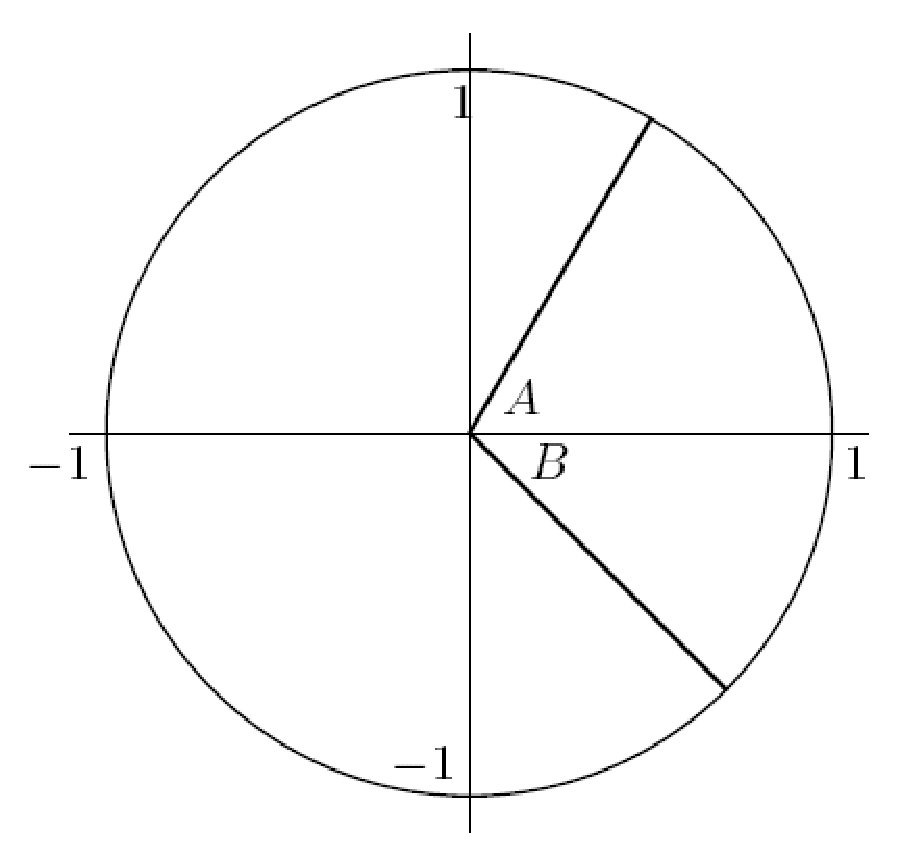
\includegraphics{SVC.01.05.005.ps}}
    \begin{center}
        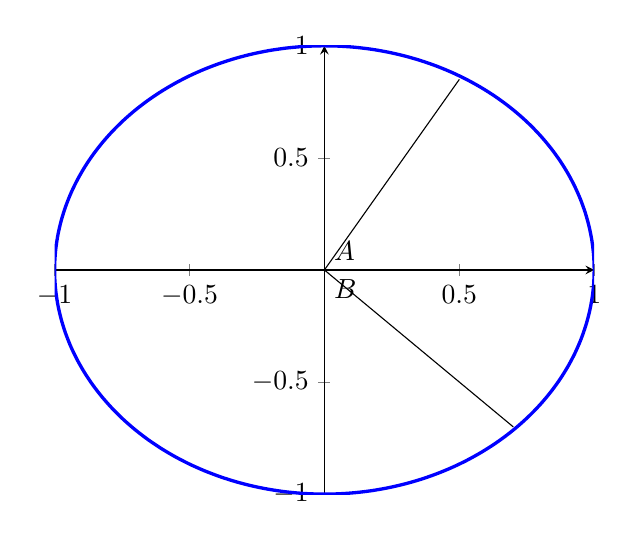
\begin{tikzpicture}
            \begin{axis}[xmin=-1, xmax=1, ymin=-1, ymax=1, axis lines = center]
                \addplot[smooth, very thick, color=blue, samples=100, domain=0:2*pi]
                ({cos(deg(x))},{sin(deg(x))});
                \draw (axis cs:0,0) node[anchor=south west]{$A$} -- (axis cs:0.5,0.85);
                \draw (axis cs:0,0) node[anchor=north west]{$B$} -- (axis cs:0.7,-0.7);
            \end{axis}
        \end{tikzpicture}
    \end{center}

\begin{enumerate}
\item $\sin A \approx 0.5$, $\cos A \approx 0.85$, $\sin B \approx -0.7$, $\cos B \approx 0.7$
\item $\sin A \approx 0.85$, $\cos A \approx 0.5$, $\sin B \approx -0.7$. $\cos B \approx 0.7$
\item $\sin A \approx 0.5$, $\cos A \approx 0.85$, $\sin B \approx 0.7$, $\cos B \approx 0.7$
\item $\sin A \approx 0.85$, $\cos A \approx 0.5$, $\sin B \approx 0.7$, $\cos B \approx 0.7$
\end{enumerate}

% ConcepTests - to accompany Calculus 4th Edition, Hughes-Hallet et al. John Wiley \& Sons.
